\documentclass[a4paper, 12pt]{article}

\usepackage[T2A]{fontenc}
\usepackage[utf8]{inputenc}
\usepackage[english,russian]{babel}
\usepackage{amsmath, amsfonts, amssymb, amsthm, mathtools}

\usepackage{indentfirst}
\usepackage{icomma}
\usepackage{hyperref}
\usepackage{soulutf8}

\usepackage{multirow}
\usepackage{hhline}
\usepackage{graphicx}

\usepackage{tikz}
\usetikzlibrary{calc}

\usepackage{diagbox}
\usepackage{wrapfig}
\usepackage{caption}
\usepackage{subcaption}

\usepackage{geometry}
\geometry{top=25mm}
\geometry{bottom=30mm}
\geometry{left=20mm}
\geometry{right=20mm}

\renewcommand{\epsilon}{\varepsilon}
\renewcommand{\phi}{\varphi}
\newcommand{\mean}[1]{\left<#1\right>}

\title{\textbf{Работа 1.2.4} \linebreak Определение главных моментов инерции твёрдых тел с помощью крутильных колебаний}
\author{Константин Ерёмин Б03-204}
\date{Ноябрь 2022}

\begin{document}
	\maketitle
	
	\section{Введение}
		\textbf{Цель:} измерить периоды крутильных колебаний рамки при различных положениях закрепленного в ней тела, проверить теоретическую зависимость между периодами крутильных колебаний тела относительно различных осей, определить моменты инерции относительно нескольких осей для каждого тела, по ним найти главные моменты инерции тел и построить эллипсоид инерции.
		
		\textbf{В работе используются:} установка для получения крутильных колебаний, набор исследуемых твёрдых тел, секундомер.
		 
	\section{Теоретическое описание работы}
		Инерционные свойства тела при вращении определяет тензор инерции, матрица которого в некоторой С.О. имеет диагональный вид. Элементы этой матрицы: $I_x$, $I_y$, $I_z$ "--- главные моменты инерции тела. Геометрический образ тензора инерции "--- эллипсоид, заданный уравнением $I_xx^2 + I_yy^2 + I_zz^2 = 1$. Знание эллипсоида инерции позволяет найти момент инерции относительно произвольной оси.

		Крутильные колебания описываются уравнением:
		\begin{equation}
			\label{eq:ostillation}
			\left(I+I_p\right)\frac{d^2\phi}{dt^2}=-f\phi
		\end{equation}
		В уравнении \ref{eq:ostillation} $I$ и $I_p$ "--- моменты инерции тела и рамки относительно оси вращения, $\phi$ "--- модуля кручения проволоки. В таком случае период крутильных колебаний можно найти по формуле:
		\begin{equation}
			\label{eq:period}
			T=2\pi\sqrt{\frac{I+I_p}{f}}
		\end{equation}

		\begin{figure}[t]
			\centering
			\begin{minipage}{0.55\textwidth}
				\centering
				\begin{tikzpicture}[scale=0.8,>=stealth]
    \coordinate[label=below:$C$] (C) at (-1, -0.5);
    \coordinate (X1) at ($(C)+(3, 2)$);
    \coordinate (X2) at ($(X1)+(-6, 0)$);
    \coordinate (X3) at ($(X2)+(0, -4)$);
    \coordinate (X4) at ($(X3)+(6, 0)$);
    \draw (X1) -- (X2) -- (X3) -- (X4) -- cycle;

    \coordinate[label=above:$C'$] (C') at (1, 0.5);
    \coordinate (Y1) at ($(C')+(3, 2)$);
    \coordinate (Y2) at ($(Y1)+(-6, 0)$);
    \coordinate (Y3) at ($(Y2)+(0, -4)$);
    \coordinate (Y4) at ($(Y3)+(6, 0)$);
    
    \draw (X4) -- (Y4) -- (Y1) -- (X1);
    \draw (X2) -- (Y2) -- (Y1);
    \draw[dashed] (Y4) -- (Y3) -- (X3);
    \draw[dashed] (Y2) -- (Y3);

    \coordinate[label=below:$A$] (A) at ($(X4)!0.5!(Y1)$);
    \coordinate[label=above:$A'$] (A') at ($(X3)!0.5!(Y2)$);
    \coordinate[label=left:$B$] (B) at ($(X1)!0.5!(Y2)$);
    \coordinate[label=right:$B'$] (B') at ($(X3)!0.5!(Y4)$);
    \draw[very thick] (C) -- (C');
    \draw[very thick] (A) -- (A');
    \draw[very thick] (B) -- (B');

    \draw[dotted,->] ($(A') + (-2,0)$) -- ($(A) + (2,0)$) node[anchor=north]{$x$};
    \draw[dotted,->] ($(B') + (0,-2)$) -- ($(B) + (0,2)$) node[anchor=west]{$y$};
    \draw[dotted,->] ($(C') + (0.8,0.4)$) -- ($(C) + (-0.8,-0.4)$) node[anchor=north]{$z$};

    \draw[thin,<->] (0,-1) ++(X3) -- ++(6,0);
    \draw ($(X3)!0.5!(X4)$) ++(0,-1) node[anchor=north]{$a$};

    \draw[thin,<->] (2,0) ++(Y4) -- ++(0,4);
    \draw ($(Y1)!0.5!(Y4)$) ++(2,0) node[anchor=west]{$b$};

    \draw[thin,<->] ($(Y4)+(2,0)$) -- ($(X4)+(2,0)$);
    \draw ($(X4)!0.5!(Y4)$) ++(2,0) node[anchor=north west]{$c$};

    \draw[thick, dash dot] ($(X2)!0.5!(X3)$) node[anchor=east]{$E$} -- ($(Y1)!0.5!(Y4)$) node[anchor=west]{$E'$};
    \draw[thick, dash dot] ($(Y1)!0.5!(Y2)$) node[anchor=south]{$M$} -- ($(X3)!0.5!(X4)$) node[anchor=north]{$M'$};
    \draw[thick, dash dot] ($(X2)!0.5!(Y2)$) node[anchor=south east]{$P$} -- ($(X4)!0.5!(Y4)$) node[anchor=north west]{$P'$};
    \draw[thick, dash dot] (X4) node[anchor=north west]{$D'$} -- (Y2) node[anchor=south east]{$D$};
\end{tikzpicture}
				\caption{Оси вращения параллелепипеда}
				\label{fig:par}
			\end{minipage}\hfill
			\begin{minipage}{0.45\textwidth}
				\centering
				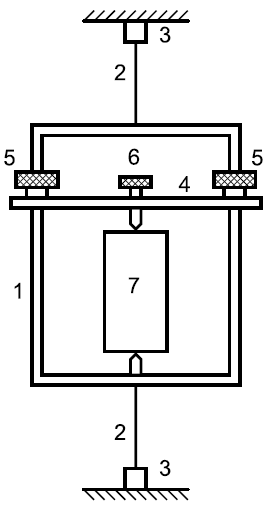
\includegraphics[width=0.45\textwidth]{setup}
				\caption{Установка}
				\label{fig:setup}
			\end{minipage}
		\end{figure}

		На рисунке \ref{fig:par} показан прямоугольный параллелепипед с главными осями $AA'$, $BB'$, $CC'$, которым соответствуют моменты инерции $I_x, I_y, I_z$. Далее приведены формулы, связывающие периоды колебаний относительно главных осей с периодами колебаний относительно некоторых других осей. Данные выражения получены с использованием формулы \ref{eq:period}, связывающей моменты инерции с периодами колебаний.

		\begin{gather}
			\left(a^2+b^2+c^2\right)T_D^2=a^2T_x^2 + b^2T_y^2 + c^2T_z^2 \\
			\left(b^2+c^2\right)T_M^2=b^2 T_y^2+c^2T_z^2 \\
			\left(a^2+c^2\right)T_E^2=a^2 T_x^2+c^2T_z^2 \\
			\left(a^2+b^2\right)T_P^2=a^2 T_x^2+b^2T_y^2
		\end{gather}

		Приведённые соотношения будут проверены экспериментально.

		\subsection*{Описание установки}
			В данной работе используется устройство для получения крутильных колебаний (рис. \ref{fig:setup}). Рамка 1 жёстко соединена с проволокой 2, закреплённой зажимами 3, задающими начальное закручивание. В рамке с помощью планки 4, гаек 5 и винта 6 закрепляется тело 7, имеющее выемки для его закрепления под различными углами.

	\section{Ход работы}
		\subsection{Измерение размеров тел}
		Перед исследованием крутильных колебаний были произведены измерения размеров тел (таблицы \ref{table:cube_size}, \ref{table:parallelepiped_size}), при этом для нахождения средних длин сторон и их погрешностей были использованы следующие формулы:
		\[\mean{d} = \frac{\sum d_i}{N} \hspace{1cm} \sigma_d = \sqrt{\frac{\sum{\left( d_i - \mean{d}\right)^2}}{N - 1}} \hspace{1cm} \sigma_{\mean{d}} = \frac{\sigma_d}{\sqrt{N}} \hspace{1cm} \sigma_\text{полн} = \sqrt{{\sigma_{\mean d}}^2 + {\Delta_d}^2} \]
		
		\begin{table}[h]
			\centering
			\begin{tabular}{|c|c|c|c|c|c|c|c|c|c|c|}
				\hline
				n & 1 & 2 & 3 & 4 & 5 & 6 & 7 & 8 & 9 & 10 \\
				\hline
				a, мм & 92.4 & 92.6 & 92.7 & 92.6 & 92.7 & 92.8 & 92.7 & 92.8 & 92.6 & 92.7 \\
				\hline
			\end{tabular}
			\caption{Измерение размеров куба}
			\label{table:cube_size}
		\end{table}

		\begin{table}
			\centering
			\begin{tabular}{|c|c|c|c|c|c|c|c|c|c|c|}
				\hline
				n & 1 & 2 & 3 & 4 & 5 & 6 & 7 & 8 & 9 & 10 \\
				\hline
				a, мм & 150.3 & 150.3 & 150.3 & 150.3 & 150.3 & 150.4 & 150.3 & 150.3 & 150.3 & 150.3 \\
				\hline
				b, мм & 100.3 & 100.4 & 100.5 & 100.3 & 100.4 & 100.4 & 100.5 & 100.5 & 100.5 & 100.4 \\
				\hline
				c, мм & 50.4 & 50.5 & 50.5 & 50.6 & 50.6 & 50.5 & 50.6 & 50.5 & 50.5 & 50.5 \\
				\hline
			\end{tabular}
			\caption{Измерение размеров параллелепипеда}
			\label{table:parallelepiped_size}
		\end{table}

		В результате были получены значения с относительной погрешностью не более 0.1\%:
		\begin{itemize}
			\item Куб: $a = 92.66 \pm 0.06$ мм
			\item Параллелепипед: $a = 150.31 \pm 0.05$ мм, $b = 100.42 \pm 0.06$ мм, $c = 50.51 \pm 0.05$ мм
		\end{itemize}

		Найдём моменты инерции тел, зная их размеры и массы ($m_\text{куб}=1085.5\pm0.05 \text{г}, m_\text{пар-д}=2081.9\pm0.05 \text{г}$), по формулам:
		\[I_x = \frac{m}{12} \left(b^2+c^2\right) \hspace{0.5cm} I_y = \frac{m}{12} \left(a^2+c^2\right) \hspace{0.5cm} I_z = \frac{m}{12} \left(a^2+b^2\right) \hspace{1cm} I_\text{куб} = \frac{ma^2}{6}\]

		\begin{itemize}
			\item Куб: $I_\text{куб} = 15.53\pm0.02 \text{ кг}\cdot\text{см}^2$
			\item Параллелепипед: $I_x = 21.92\pm0.03 \text{ кг}\cdot\text{см}^2, I_y = 43.62\pm0.06\text{ кг}\cdot\text{см}^2, I_z = 56.65\pm0.08\text{ кг}\cdot\text{см}^2$
		\end{itemize}

		Тогда для параллелепипеда получаем следующие отношения моментов инерции главных осей:
		\[I_y:I_x = 2.000\pm0.004\hspace{1cm} I_z:I_y = 1.299\pm0.003\hspace{1cm} I_z:I_x = 2.584\pm0.005\]

		\subsection{Измерение периодов колебаний}
		Далее было проведено знакомство с установкой и была проверена корректность ей работы: крепление проволоки, работа устройства для возбуждения колебаний, усточивость крутильных колебаний.

		Затем измерялись периоды колебаний куба и параллелепипеда вокруг различных осей. Период считался по времени 12 колебаний. Результаты можно увидеть в таблицах \ref{table:cube} и \ref{table:parallelepiped}. Погрешность определения периода оценим так: абсолютная погрешность измерения составляет $0.3$ с (скорость реакции), так что $\epsilon_T = \frac{0.3}{12T} \sim \frac{0.3}{12} \approx 0.03 = 3\%$.

		\begin{table}[h]
			\centering
			\begin{tabular}{|c|c|c||c|c|c|}
				\hline
				\diagbox[width=1.6cm]{n}{T, с} & $T^\text{р}$ & $T_{1/2}^\text{р}$ & $T_\text{г.о.}^\text{к}$ & $T_D^\text{к}$ & $T_E^\text{к}$ \\
				\hline
				1 & 2.56 & 2.56 & 3.03 & 3.01 & 3.01 \\
				\hline
				2 & 2.55 & 2.58 & 3.05 & 3.07 & 3.02 \\
				\hline
				3 & 2.63 & 2.57 & 3.06 & 3.03 & 3.04 \\
				\hline\hline
				$\mean{T}$, с & 2.58 & 2.57 & 3.05 & 3.04 & 3.02 \\
				\hline
			\end{tabular}
			\caption{Измерения периодов колебаний рамки и куба}
			\label{table:cube}
		\end{table}

		\begin{table}[h]
			\centering
			\begin{tabular}{|c|c|c|c|c|c|c|c|}
				\hline
				\diagbox[width=1.6cm]{n}{T, с} & $T_A$ & $T_B$ & $T_C$ & $T_E$ & $T_M$ & $T_P$ & $T_D$ \\
				\hline
				1 & 3.18 & 3.7 & 3.98 & 3.28 & 3.76 & 3.35 & 3.4 \\
				\hline
				2 & 3.18 & 3.73 & 3.98 & 3.28 & 3.78 & 3.36 & 3.41 \\
				\hline
				3 & 3.2 & 3.7 & 3.97 & 3.31 & 3.77 & 3.4 & 3.41 \\
				\hline\hline
				$\mean{T}$, с & 3.19 & 3.71 & 3.98 & 3.29 & 3.77 & 3.37 & 3.41 \\
				\hline
			\end{tabular}
			\caption{Измерения периодов колебаний параллелепипеда}
			\label{table:parallelepiped}
		\end{table}

		\subsection{Проверка теоретической зависимости}
		Проверим теоретическую связь между размерами тела и периодами колебаний:		
		\begin{gather*}
			\left(a^2+b^2+c^2\right)T_D^2=a^2T_x^2 + b^2T_y^2 + c^2T_z^2 \\
			\left(b^2+c^2\right)T_M^2=b^2T_y^2+c^2T_z^2 \\
			\left(a^2+c^2\right)T_E^2=a^2T_x^2+c^2T_z^2 \\
			\left(a^2+b^2\right)T_P^2=a^2T_x^2+b^2T_y^2
		\end{gather*}

		\begin{wraptable}{c}{5cm}
			\centering
			\begin{tabular}{|c|c|c|}
				ось & $\Delta$ & $\sigma_\Delta$ \\
				\hline
				$DD'$ & 514 & 8722 \\
				$MM'$ & 372 & 3685 \\
				$EE'$ & 1837 & 6611 \\
				$PP'$ & 2403 & 8209
			\end{tabular}
			\caption{Проверка теории (размерности: $\text{мм}^2 \cdot \text{с}^2$)}
			\label{table:check}
		\end{wraptable}
 
		Для этого из левой части каждого равенства вычтем правую, и, пренебрегая погрешностью измерения размеров тела по сравнению с погрешностью периода колебаний, получим погрешность разности по формуле:
		\[\sigma^2 = \left(\left(a^2 + b^2\right) 2T_M \sigma_M\right)^2 + \left(a^2 2T_x \sigma_x\right)^2 + \left(b^2 2T_y \sigma_y\right)^2\]
		для последнего равенства (для остальных формула аналогичная). Полученные разности и их погрешности занесены в таблицу \ref{table:check}. Все разности оказались в пределах погрешностей, так что можно считать теоретические соотношения верными.

		\subsection{Построение эллипсоида инерции}
			Для осей в главных плоскостях вычислим величину $1/\sqrt{T^2-T_\text{р}^2}$, пропорциональную расстоянию от центра масс тела до точки пересечения эллипсоида с этой осью. В соответствующих координатах изобразим эллипсоид инерции параллелепипеда и куба (рис. \ref{fig:parped} и \ref{fig:cube_el}). По длинам осей эллипсоидов находятся отношения между моментами инерции.

			\begin{figure}[h]
				\centering
				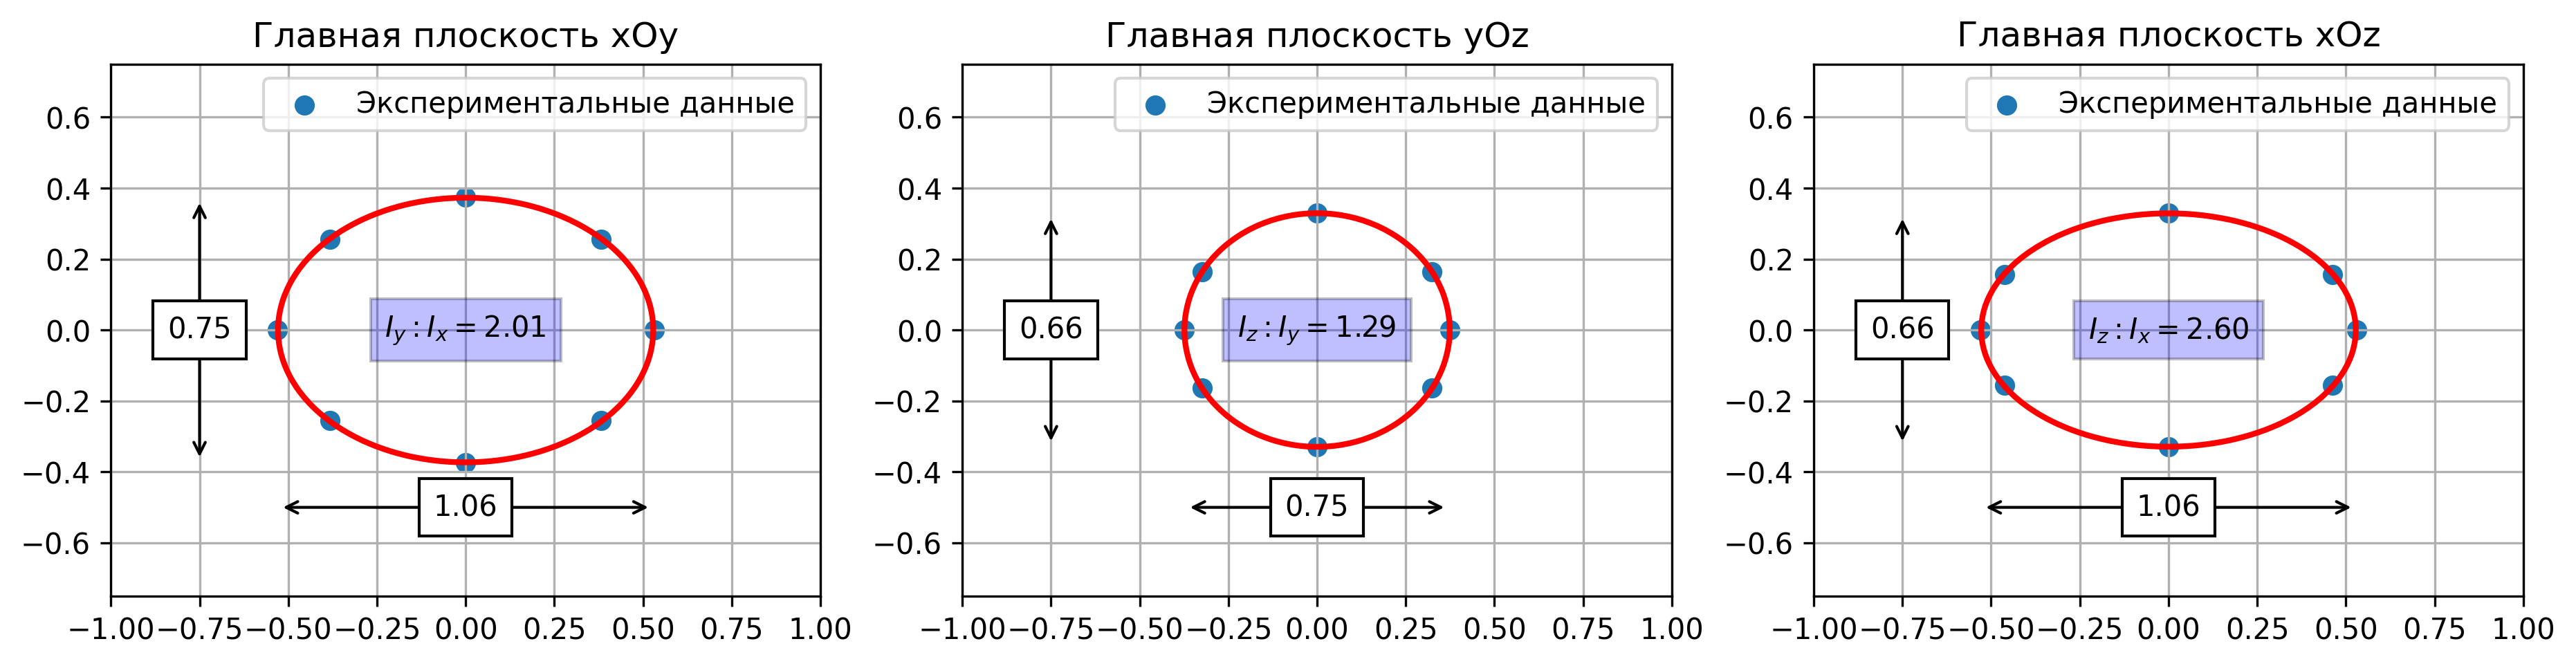
\includegraphics[width=\linewidth]{parped.png}
				\caption{Эллипсоид инерции параллелепипеда}
				\label{fig:parped}
			\end{figure}
			\begin{figure}[h]
				\centering
				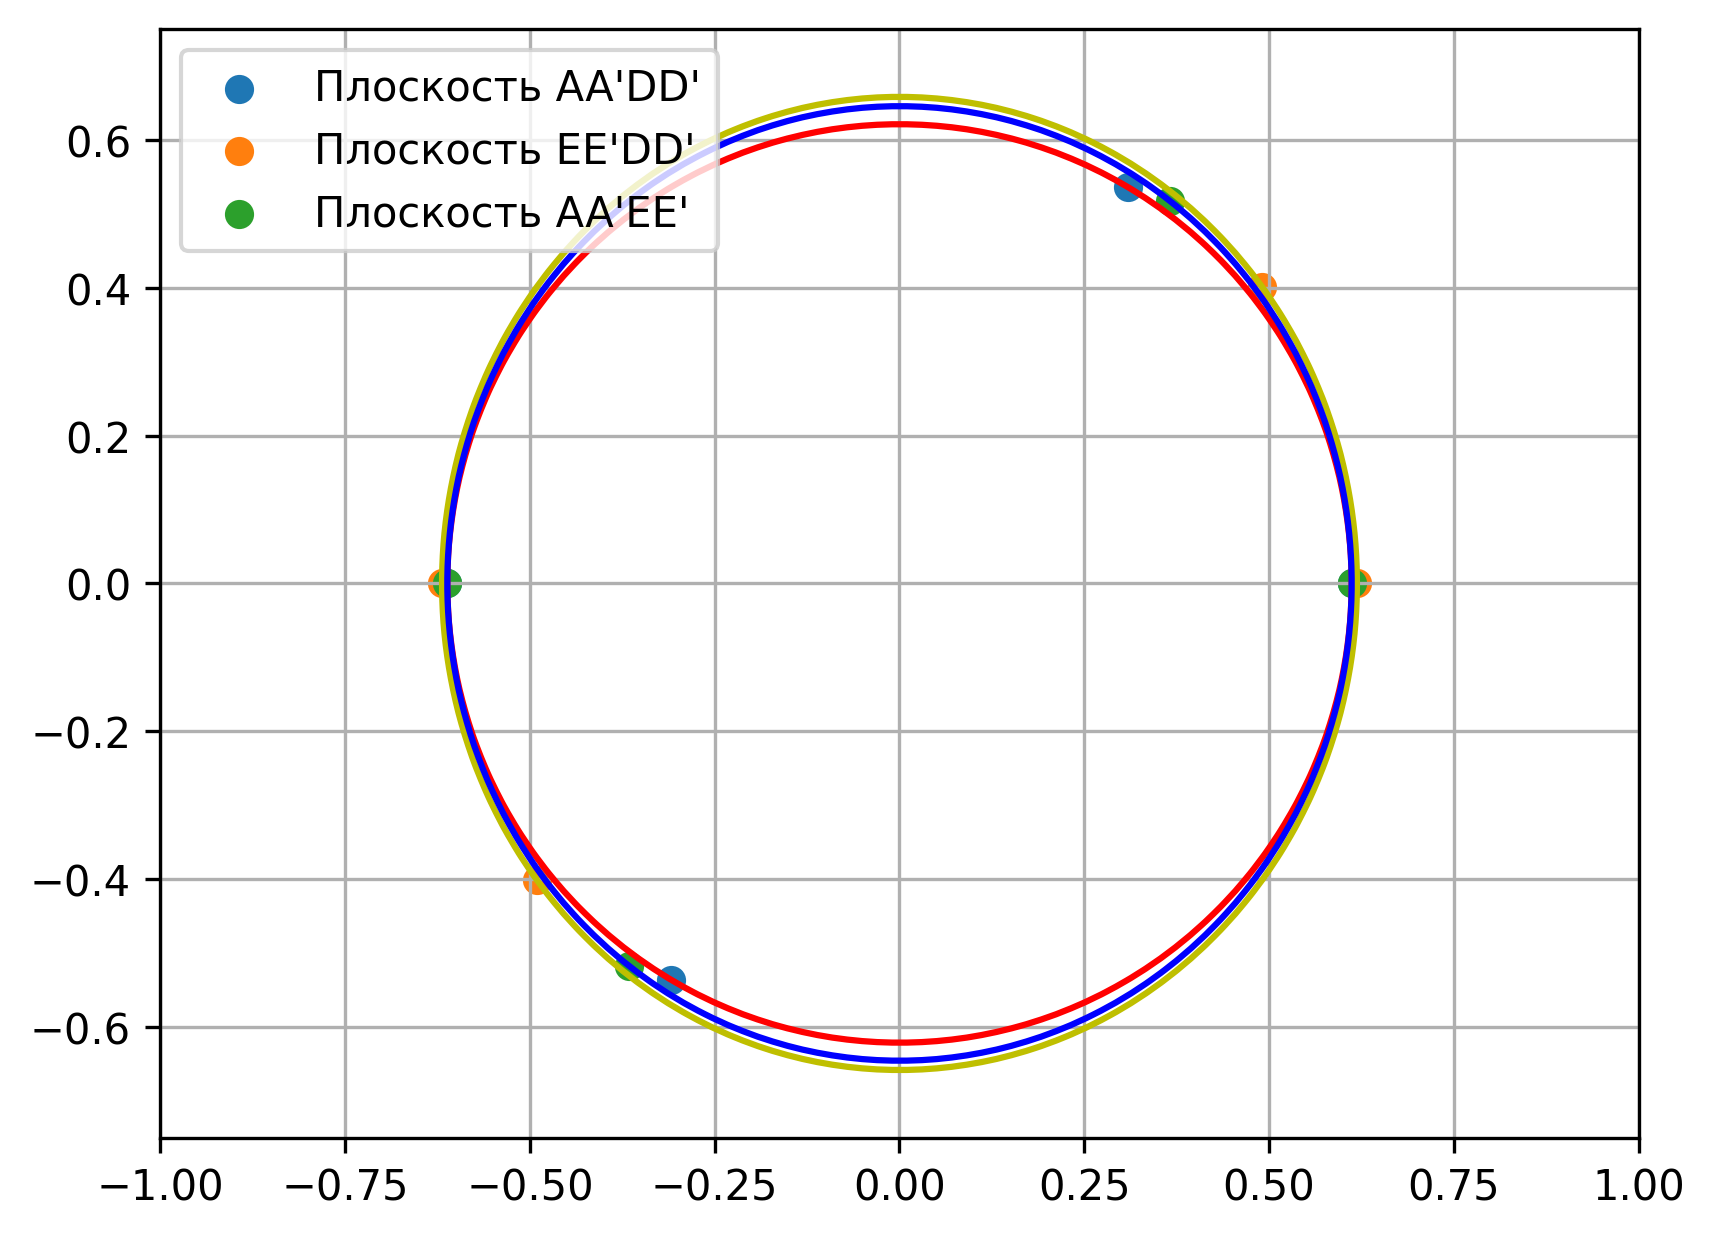
\includegraphics[width=0.8\linewidth]{cube.png}
				\caption{Эллипсоид инерции куба}
				\label{fig:cube_el}
			\end{figure}
	\section{Вывод}
		В ходе работы были проверены некоторые теоретические соотношения теории крутильных колебаний и построены эллипсоиды инерции, с помощью которых затем была подтверждена правильность расчётов моментов инерции относительно различных осей тел. 
\end{document}